\documentclass[12pt, a4paper]{article}

% Preamble
\usepackage{xeCJK}
\usepackage[utf8]{inputenc}
\usepackage[english]{babel}
\usepackage[margin=1in]{geometry}
\usepackage[parfill]{parskip}
\usepackage{listings}
\usepackage{graphics}
\usepackage{graphicx}
\usepackage{nasm/lang}
\usepackage{nasm/style}
\usepackage{c/style}
\usepackage{go/lang}
\usepackage{go/style}
\usepackage{reil/lang}
\usepackage{llvm/lang}
\usepackage{diff/lang}
\usepackage{diff/style}
\usepackage{dot/lang}
\usepackage{dot/style}
\usepackage{float}
\usepackage[colorlinks,linkcolor=blue]{hyperref}


% Document

\usepackage{etoolbox}
\makeatletter
\def\@xobeysp{\hspace{0pt}\mbox{ }\hspace{0pt}}
\appto\verbatim@font{\hyphenchar\font`-\relax}
\apptocmd\@sverb{\hspace*{0pt}}{}{}
\makeatother

\title{COD\_LAB2 数据通路与状态机}
\author{黄业琦 PB17000144}
\date{March 25, 2019}
\begin{document}
\maketitle
\tableofcontents
\clearpage
\definecolor{vgreen}{RGB}{104,180,104}
\definecolor{vblue}{RGB}{49,49,255}
\definecolor{vorange}{RGB}{255,143,102}
\lstdefinestyle{verilog-style}
{
	language=Verilog,
	basicstyle=\small\ttfamily,
	keywordstyle=\color{vblue},
	identifierstyle=\color{black},
	commentstyle=\color{vgreen},
	numbers=left,
	numberstyle=\tiny\color{black},
	numbersep=7pt,
	tabsize=4,
	literate=*{:}{{\textcolor{black}{:}}}1
}
\section{实验目的}
\subsection{排序}
s0 - s3是x0 - x3的排序结果。
\begin{figure}[H]
	\centering
	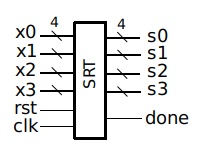
\includegraphics[width=0.4\linewidth]{sort}
	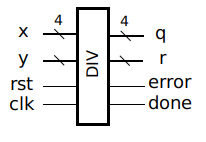
\includegraphics[width=0.4\linewidth]{div}
	\caption{Sort \& Div}
	\label{Sort}
\end{figure}
\subsection{除法运算}
x / y = q … r
\clearpage

\section{实验环境}
Linux下编程调试和仿真,使用IVerilog,GtkWave系列工具。\\
Windows下用于生成比特流文件,使用Vivado 2018.2,Verilog HDL\\
所有下载均在Nexsy4-DDR实验板完成

\section{逻辑设计}
\subsection{Sort设计}
采用六次比较以实现我们的排序工作。\\
详细见附录代码。
\subsection{Fibonacci设计和累计求和}
采用移位算法实现我们的除法操作:\\
1、被除数为x,除数为y,商为qout,余数为rout;\\
2、将被除数赋给寄存器变量q,变量r初始值为0,t为{q,r};\\
3、先将t左移一位;\\
4、比较r与除数的大小,如果r>除数则r=r-除数并且t再左移一位并且q[0]=1,反之r不变t左移一位q[0]=0。\\
5、继续上述过程,循环至无法移位了;\\
6、此时商qout=q,而余数rout=r>>1(即余数等于r向右移一位)。\\
\clearpage

\section{仿真截图}
\begin{figure}[H]
	\centering
	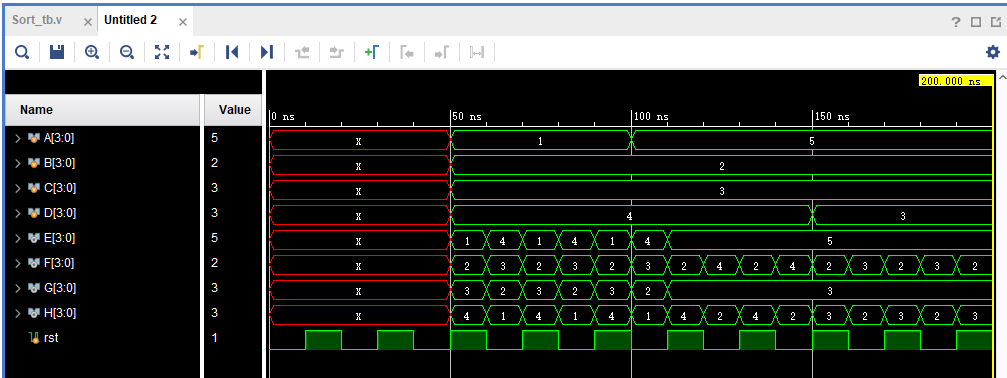
\includegraphics[width=1.0\linewidth]{/home/chivier_humber/Documents/Study/COD_LAB/LAB2/SORT_sim.PNG}
	\caption{SORT\_sim}
\end{figure}
\begin{figure}[H]
\centering
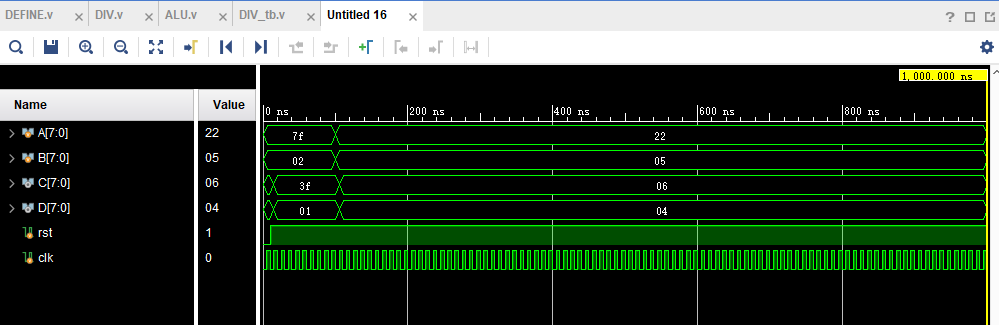
\includegraphics[width=1.0\linewidth]{/home/chivier_humber/Documents/Study/COD_LAB/LAB2/DIV_sim.PNG}
\caption{DIV\_sim}
\end{figure}
\clearpage

\section{性能评测截图}
\begin{figure}[H]
	\centering
	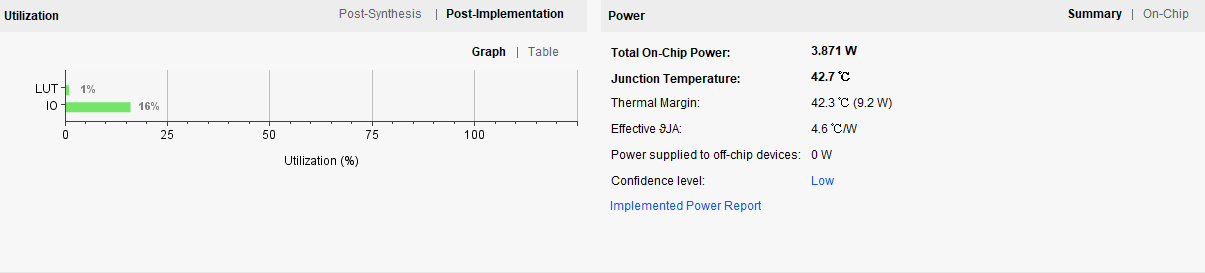
\includegraphics[width=1.0\linewidth]{/home/chivier_humber/Documents/Study/COD_LAB/LAB2/Sort_Performance1.PNG}
	\caption{Sort\_Performance1}
\end{figure}
\begin{figure}[H]
	\centering
	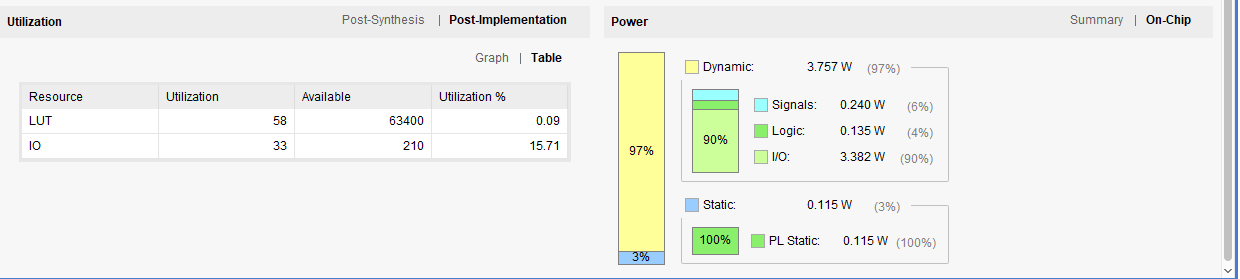
\includegraphics[width=1.0\linewidth]{/home/chivier_humber/Documents/Study/COD_LAB/LAB2/Sort_Performance2.PNG}
	\caption{Sort\_Performance2}
\end{figure}
\begin{figure}[H]
	\centering
	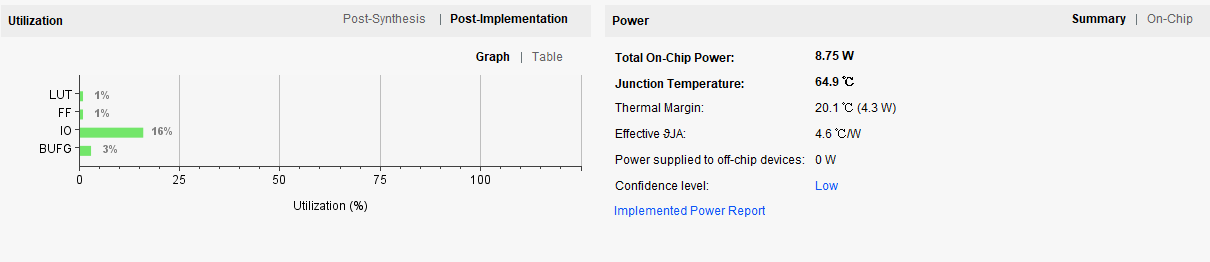
\includegraphics[width=1.0\linewidth]{/home/chivier_humber/Documents/Study/COD_LAB/LAB2/DIV_Performance1.PNG}
	\caption{DIV\_Performance1}
\end{figure}
\begin{figure}[H]
	\centering
	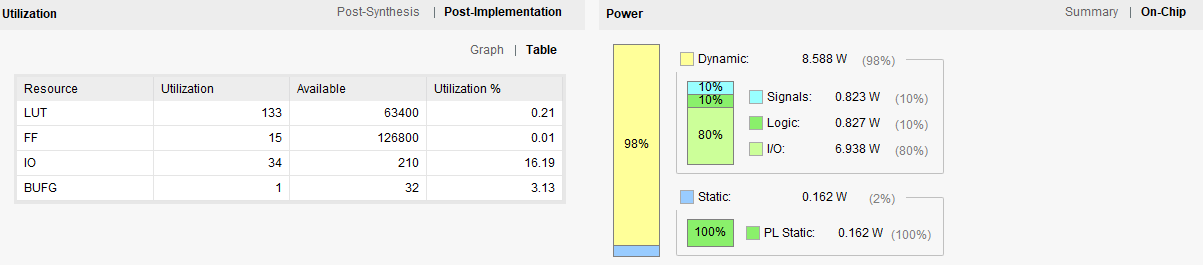
\includegraphics[width=1.0\linewidth]{/home/chivier_humber/Documents/Study/COD_LAB/LAB2/DIV_Performance2.PNG}
	\caption{DIV\_Performance2}
\end{figure}
\clearpage

\section{实验代码}
\subsection{Sort实现代码}
DEFINE和ALU同上一次的实验,不再重复给出。
\lstinputlisting[style={verilog-style},caption={CMP.v}]{/home/chivier_humber/Documents/Study/COD_LAB/LAB2/Sort/Sort.srcs/sources_1/new/CMP.v}
\lstinputlisting[style={verilog-style},caption={Sort.v}]{/home/chivier_humber/Documents/Study/COD_LAB/LAB2/Sort/Sort.srcs/sources_1/new/Sort.v}
\lstinputlisting[style={verilog-style},caption={Sort\_tb.v}]{/home/chivier_humber/Documents/Study/COD_LAB/LAB2/Sort/Sort.srcs/sim_1/new/Sort_tb.v}
\subsection{DIV实现代码}
\lstinputlisting[style={verilog-style},caption={DIV.v}]{/home/chivier_humber/Documents/Study/COD_LAB/LAB2/DIV/DIV.srcs/sources_1/new/DIV.v}
\lstinputlisting[style={verilog-style},caption={DIV\_tb.v}]{/home/chivier_humber/Documents/Study/COD_LAB/LAB2/DIV/DIV.srcs/sim_1/new/DIV_tb.v}

\section{FSM实现}
\subsection{排序 FSM设计}
我们设计存在三个状态:
\begin{enumerate}
	\item 初始状态,加载数据
	\item 一趟排序流程(冒泡一趟)
	\item 终
\end{enumerate}

\begin{figure}[H]
	\centering
	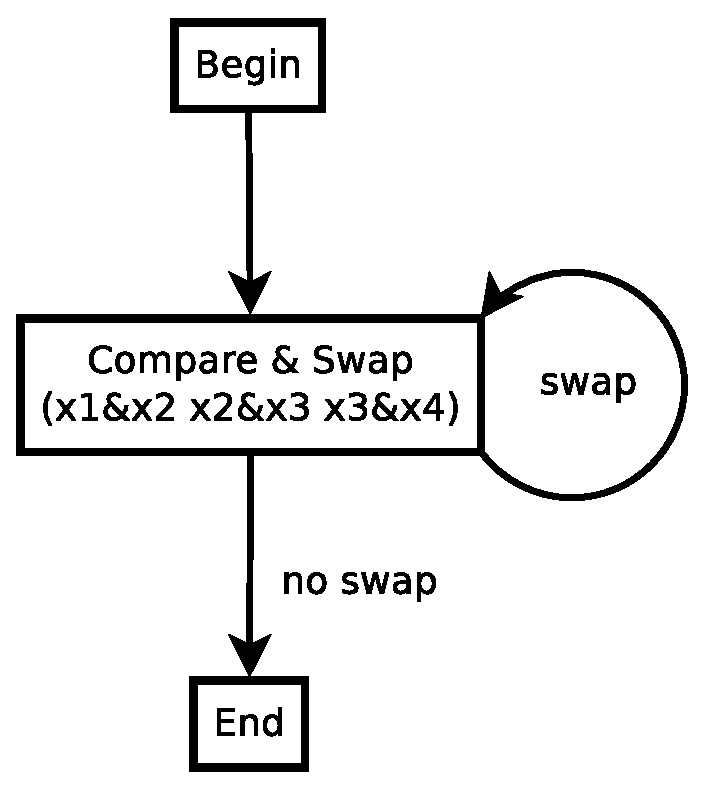
\includegraphics[width=0.4\linewidth]{sortfsm.eps}
	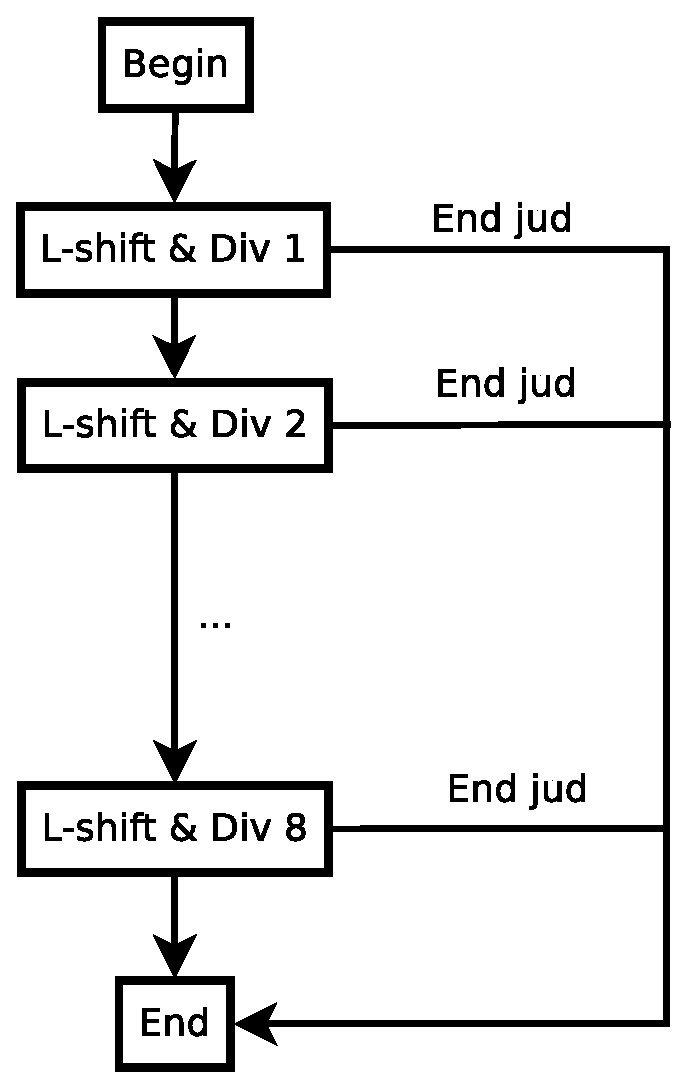
\includegraphics[width=0.4\linewidth]{divfsm.eps}
	\caption{Sort \& Div}
	\label{FSM}
\end{figure}

\subsection{除法 FSM设计}
我们设计存在三个状态:
\begin{enumerate}
	\item 初始状态,加载数据
	\item 一趟移位除法操作,同之前算法描述处介绍
	\item 终
\end{enumerate}
之前的i循环变量视为状态编号就可以将之前的代码视作两段式状态机的程序。

\section {三段式状态机代码}
仿真图像和之前一致,不再重复给出。这里在DivFSM中加入了err判定以及我们的Done判定。(之前写漏了)
\subsection{SortFSM实现代码}
\lstinputlisting[style={verilog-style},caption={Sort.v}]{/home/chivier_humber/Desktop/Study/COD_LAB/LAB2/sortfsmcode.v}
\lstinputlisting[style={verilog-style},caption={Seg\_out.v}]{/home/chivier_humber/Desktop/Study/COD_LAB/LAB2/SegOUT.v}

\end{document}